\chapter{Μετασχηματισμοί στο Επίπεδο – Παραστάσεις με Πίνακες}
		
Στο κεφάλαιο αυτό θα ασχοληθούμε με τα δύο είδη μετασχηματισμών, δηλαδή τους βασικούς μετασχηματισμούς αξόνων συντεταγμένων και τους βασικούς γεωμετρικούς μετασχηματισμούς. Οι αντίστοιχοι μετασχηματισμοί των δύο παραπάνω κατηγοριών είναι:

\begin{center}
\begin{tabular}{m{0.45\textwidth}m{0.45\textwidth}}
\toprule
\textbf{Μετασχηματισμοί αξόνων} & \textbf{Γεωμετρικοί μετασχηματισμοί} \\
\midrule
1. Μεταφορά αρχής. & 1. Μεταφορά σχήματος. \\
2. Αλλαγή κλίμακας αξόνων συντεταγμένων. & 2. Αλλαγή κλίμακας συντεταγμένων, σχετικά με την παράσταση ενός αντικειμένου (μεγέθυνση – σμίκρυνση). \\
3. Στροφή των αξόνων συντεταγμένων. & 3. Στροφή σχήματος γύρω από την αρχή των αξόνων. \\
4. Συμμετρία ως προς άξονα. & 4. Συμμετρία ως προς άξονα. \\
5. Αντίστροφοι των 1 έως 4 μετασχηματισμοί. & 5. Αντίστροφοι των 1 έως 4 μετασχηματισμοί. \\
\bottomrule
\end{tabular}
\end{center}


Μέχρι τώρα θεωρούσαμε ότι η αρχή των αξόνων, οι άξονες καθώς και η κλίμακα επί των αξόνων, συμπίπτουν με την αρχή, τους άξονες και την κλίμακα της οθόνης. Το σύστημα συντεταγμένων της οθόνης καλείται και σύστημα του παρατηρητή. Γενικά δεν υπάρχει σύμπτωση του αρχικού (πραγματικού) συστήματος με το σύστημα του παρατηρητή. Τέλος, ο όρος \textquotedblleft βασικοί μετασχηματισμοί\textquotedblright\ προκύπτει από τη δυνατότητα κάθε άλλος μετασχηματισμός να μπορεί να αντιμετωπιστεί με συνδυασμό των αντίστοιχων βασικών μετασχηματισμών.

\section{Βασικοί μετασχηματισμοί αξόνων συντεταγμένων}

\subsection{Παράλληλη μεταφορά αρχής συντεταγμένων}

Έστω \((t_x, t_y)\) οι συντεταγμένες της νέας αρχής σχετικά με την παλαιά. Στο νέο σύστημα οι συντεταγμένες αρχής του παλαιού είναι \((-t_x, -t_y)\). Άρα για το σημείο \(P(x, y)\) θα έχουμε σαν συντεταγμένες του στο σύστημα \(x'Oy'\) τις εξής:
%
\[
(x' = x - t_x, \, y' = y - t_y).
\]

\begin{figure}[hbt]
  \begin{center}
	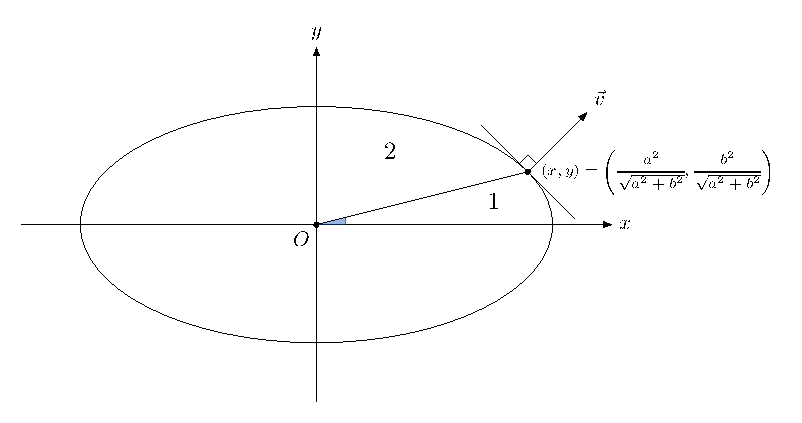
\includegraphics[scale=1]{Chapter2/figure1.pdf}
  \end{center}
  \caption{Παράλληλη μεταφορά αρχής συντεταγμένων}
\end{figure}




\begin{lstlisting}
# Parrallel metafora	
\end{lstlisting}





\begin{tabular}{m{0.45\textwidth}m{0.45\textwidth}}
	Συμβολισμός μετασχηματισμού: & $ \bar{T}_\mathbf{v} $\\
	Επομένως έχουμε: & $(x', y') = \bar{T}_\mathbf{v}(x, y)$\\
	όπου & $x' = x - t_x$ και $y' = y - t_y$
\end{tabular}


\section{Αλλαγή κλίμακας αξόνων συντεταγμένων}

Θεωρώντας ότι το σύστημα συντεταγμένων δεν αλλάζει ούτε σε θέση ούτε σε διεύθυνση μπορούμε να αλλάξουμε τις μονάδες μέτρησης κατά μήκος των δύο αξόνων. Έστω $S_x$ και $S_y$ οι ``κλίμακες'' (παράγοντες) βάσει των οποίων προκύπτουν, οι νέες μονάδες μέτρησης.
 
 
\begin{tabular}{m{0.45\textwidth}m{0.45\textwidth}}
	Συμβολισμός μετασχηματισμού: & $ \bar{S}_{S_x, S_y}$\\
	Επομένως έχουμε: & $(x', y') = \bar{S}_{S_x, S_y}(x, y)$\\
	όπου & $x' = \cfrac{1}{S_x} x$ και $y' = \cfrac{1}{S_y} y$.
\end{tabular}


\begin{figure}[h!]
\begin{center}
	\begin{minipage}[b]{0.48\textwidth} % Top-left image
	    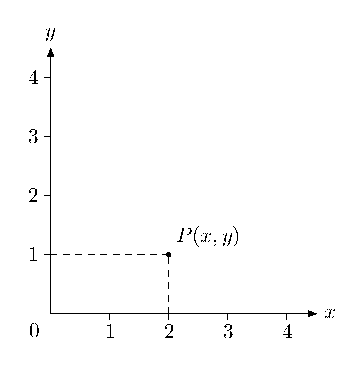
\includegraphics[width=\textwidth]{Chapter2/figure2a.pdf}
	%    \captionof{figure}{Top-Left Image}
	\end{minipage}%
	\hfill
	\begin{minipage}[b]{0.48\textwidth} % Top-right image
	    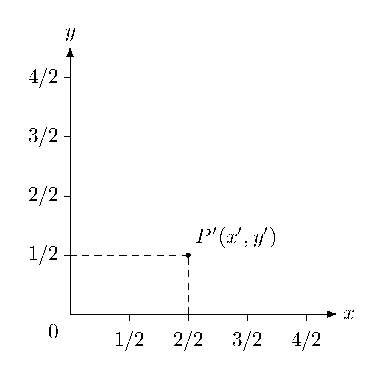
\includegraphics[width=\textwidth]{Chapter2/figure2b.pdf}
	%    \captionof{figure}{Top-Right Image}
	\end{minipage}
\end{center}
  \caption{Παράδειγμα αλλαγής κλίμακας αξόνων συντεταγμένων για $S_x = 2$ και $S_y = 2$.}
\end{figure}


\begin{lstlisting}
# Allagi klimakas ajwnwn
\end{lstlisting}



\subsection{Στροφή των αξόνων συντεταγμένων}
Έστω ότι το σύστημα $xOy$ στρέφει κατά γωνία $\theta$ γύρω από το $O$.

\begin{figure}[hbt]
  \begin{center}
	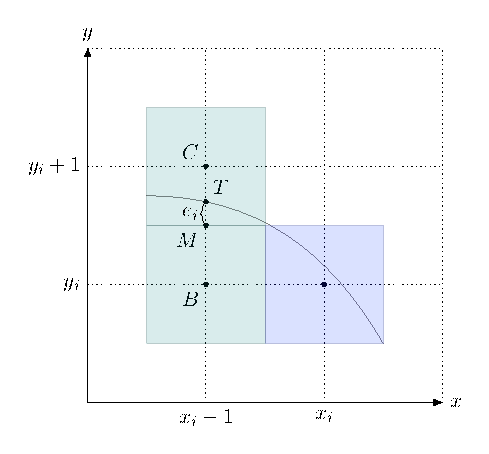
\includegraphics[scale=1.2]{Chapter2/figure3.pdf}
  \end{center}
  \caption{Στροφή συστήματος αξόνων κατά γωνία $\theta$ γύρω από την αρχή των αξόνων $O$.}
\end{figure}

\begin{figure}[h!]
  \begin{center}
	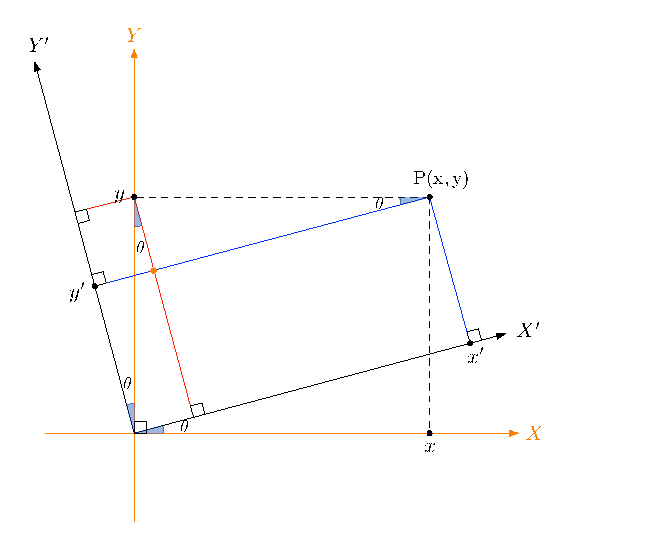
\includegraphics[scale=0.9]{Chapter2/axis-rotation.pdf}
  \end{center}
  \caption{Στροφή συστήματος αξόνων κατά γωνία $\theta$ γύρω από την αρχή των αξόνων $O$.}
\end{figure}


\begin{lstlisting}
# strofi systimatos ajwnwn
\end{lstlisting}

 % Adjust this number to increase line spacing
\begin{tabular}{m{0.45\textwidth}m{0.45\textwidth}}
	Συμβολισμός μετασχηματισμού: & $ \bar{R}_\theta $\\
	Επομένως: & $(x', y') = \bar{R}_\theta (x, y)$\\
\end{tabular}

\textcolor{red}{ΝΑ μπουν τα B' κλπ στο σχήμα}
Από το σχήμα έχουμε ότι 
\[
	OB' = y \sin\theta \quad \text{και} \quad B'X'' = x \cos\theta
\]

Άρα $x' = OX = OB' + B'X = x \cos\theta + y \sin\theta$.
Άρα $y' = OY = A'O - A'Y = y \cos\theta - x \sin\theta$.

\subsection{Συμμετρία ως προς άξονα}


\begin{tabular}{m{0.45\textwidth}m{0.45\textwidth}}
	Συμβολισμός μετασχηματισμού: & $ \bar{M}_x $\\
	Επομένως: & $(x',y') = \bar{M}_x(x,y) \text{ όπου } x' = x, y' = -y$\\
	& $(x',y') = \bar{M}_y(x,y) \text{ όπου } x' = -x, y' = y$
\end{tabular}


\begin{figure}[h!]
\begin{center}
\begin{minipage}[b]{0.48\textwidth} % Top-left image
    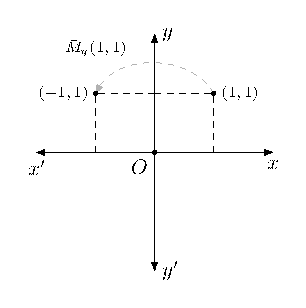
\includegraphics[width=\textwidth]{Chapter2/figure4a.pdf}
%    \captionof{figure}{Top-Left Image}
\end{minipage}%
\hfill
\begin{minipage}[b]{0.48\textwidth} % Top-right image
    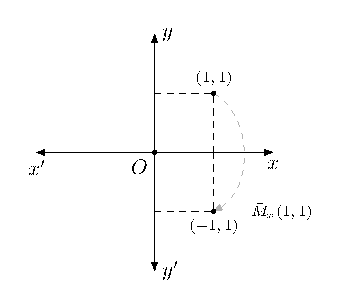
\includegraphics[width=\textwidth]{Chapter2/figure4b.pdf}
%    \captionof{figure}{Top-Right Image}
\end{minipage}

\end{center}
  \caption{Παράδειγμα συμμετρίας ως προς άξονα}
\end{figure}

\subsection{ Αντίστροφοι μετασχηματισμοί αξόνων συντεταγμένων}


\begin{tabular}{m{0.6\textwidth}m{0.45\textwidth}}
	Μεταφορά (μεταφορά στην αντίθετη κατεύθυνση): & $ \bar{T}_v^{-1} = \bar{T}_{-v} $\\
	Κλίμακα: & $\bar{S}_{S_x, S_y}^{-1} = \bar{S}_{\cfrac{1}{S_x}, \cfrac{1}{S_y}}$\\
	Στροφή(στροφή στην αντίθετη κατεύθηνση):& $ \bar{R}_\theta^{-1} = \bar{R}_{-\theta} $\\
	Συμμετρία: & $\bar{M_x}^{-1} = \bar{M_x} \quad \text{και} \quad \bar{M_y}^{-1} = \bar{M_y}$
\end{tabular}




\section{Βασικοί γεωμετρικοί μετασχηματισμοί.}

Στους γεωμετρικούς μετασχηματισμούς πρόκειται ουσιαστικά για ``αλλαγή της θέσης" στην οποία βρίσκεται ένα επίπεδο σχήμα, θεωρώντας τους άξονες και γενικά το σύστημα συντεταγμένων σταθερό.

\subsection{Μεταφορά σχήματος}

\begin{figure}[h!]
\begin{center}
\begin{minipage}[b]{0.48\textwidth} % Top-left image
    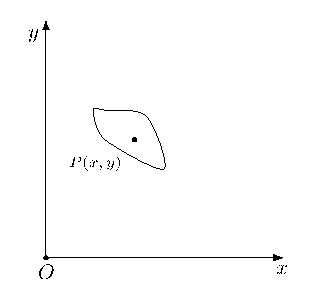
\includegraphics[width=\textwidth]{Chapter2/figure5a.pdf}
%    \captionof{figure}{Top-Left Image}
\end{minipage}%
\hfill
\begin{minipage}[b]{0.48\textwidth} % Top-right image
    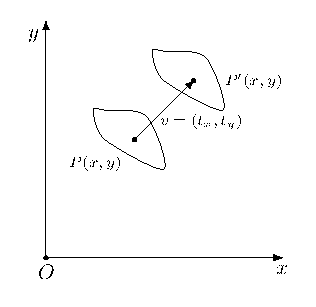
\includegraphics[width=\textwidth]{Chapter2/figure5b.pdf}
%    \captionof{figure}{Top-Right Image}
\end{minipage}

\end{center}
  \caption{Παράδειγμα μεταφοράς σχήματος κατά διάνυσμα $v = (t_x, t_y)$}
\end{figure}

Συμβολισμός: $T_v : P' = T_v(P)$ όπου $x' = x + t_x$ και $y' = y + t_y$.

\subsection{Αλλαγή κλίμακας (Μεγέθυνση - σμίκρυνση)}

Ο μετασχηματισμός κλίμακας είναι εδώ μια διαδικασία ``μεγέθυνσης" ή ``σμίκρυνσης" των διαστάσεων ενός σχήματος. Κρατώντας σταθερή την αρχή και τους άξονες δίνουμε μία μεγέθυνση όλης της περιοχής του σχήματος κατά $S_x$ στη διεύθυνση του θετικού άξονα $x$ και αντίστοιχα κατά $S_y$ στη διεύθυνση του θετικού άξονα $y$. Φυσικά επειδή εδώ πρόκειται για μεγέθυνση ισχύει $S_x > 1$ και $S_y > 1$. Αντίθετα όταν πρόκειται για σμίκρυνση έχουμε $S_x < 1$ και $S_y < 1$. Τέλος υπάρχουν και συνδυασμοί των τεσσάρων περιπτώσεων.

Συμβολισμός μετασχηματισμού: $S_{S_x, S_y} : P' = S_{S_x, S_y}(P)$ όπου $x' = S_x \cdot x$ και $y' = S_y \cdot y$.


Παράδειγμα για $S_x = 2$ και $S_y = \cfrac{1}{2}$:

\begin{figure}[h!]
	\begin{center}
		\begin{minipage}[b]{0.48\textwidth}
		    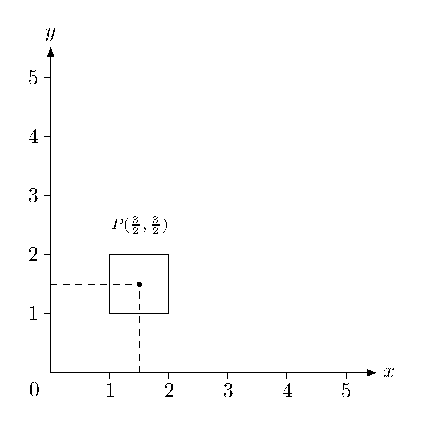
\includegraphics[width=\textwidth]{Chapter2/figure6a.pdf}
		\end{minipage}
		\hfill
		\begin{minipage}[b]{0.48\textwidth} 
		    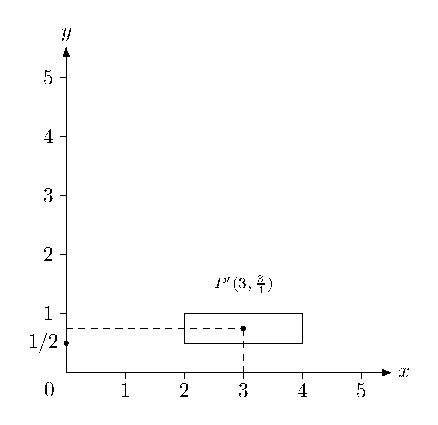
\includegraphics[width=\textwidth]{Chapter2/figure6b.pdf}
		\end{minipage}
	\end{center}
	\caption{Παράδειγμα αλλαγής κλίμακας συντεταγμένων (Σμίκρυνση στον $y$ και μεγέθυνση στον $x$)}
\end{figure}

\begin{remark}
	Σε αυτό το μετασχηματισμό \underline{το μόνο σημείο που δεν μετασχηματίζεται}\\ \underline{είναι η αρχή των αξόνων}.	
\end{remark}


\subsection{Στροφή σχήματος γύρω από την αρχή των αξόνων}


\begin{figure}[h!]
	\begin{center}
	    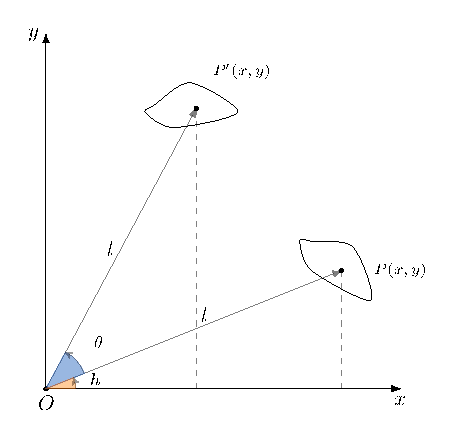
\includegraphics[scale=1]{Chapter2/figure7.pdf}
	\end{center}
	\caption{Στροφή σχήματος γύρω από την αρχή των αξόνων κατά γωνία $\theta$}
\end{figure}


\begin{tabular}{m{0.4\textwidth}m{0.5\textwidth}}
	Συμβολισμός μετασχηματισμού: & $R_\theta$ και επομένως $P'=R_\theta(P)$ με :\\
	& $x = l \cosh \, \, l = \sqrt{x^2 + y^2}, \, y = l \sinh \,$\\
	Άρα τελικά :& $x' = l \cos(\theta + h) = l(\cosh \cos \theta - \sinh \sin \theta) = x \cos \theta - y \sin \theta$\\
\end{tabular}

Ομοίως προκύπτει ότι $y' = x \sin \theta + y \cos \theta$.

\subsection{Συμμετρία ως προς άξονα}


\begin{tabular}{m{0.4\textwidth}m{0.5\textwidth}}
	Συμβολισμός μετασχηματισμού: & $M_x, M_y$\\
	& $P' = M_x(P)$ όπου $x' = x$ και $y' = -y$\\
	& $ P' = M_y(P)$  όπου $x' = -x $ και $ y' = y.$  \\
\end{tabular}


Τη \underline{συμμετρία} μπορούμε εδώ να τη θεωρήσουμε \underline{σαν μετασχηματισμό κλίμακας} με \underline{$S_x = 1, S_y = -1$} για την περίπτωση  \underline{$M_x$  και  $S_x = -1, S_y = 1$ για την  $M_y.$}

\begin{figure}[h!]
	\begin{center}
	    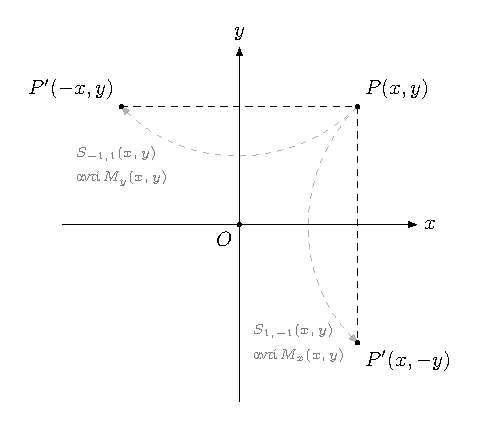
\includegraphics[scale=1]{Chapter2/figure8.pdf}
	\end{center}
	\caption{Παραδείγματα συμμετρίας σημείου ως προς άξονες}
\end{figure}


\subsection{Αντίστροφοι γεωμετρικοί μετασχηματισμοί}


\begin{tabular}{m{0.2\textwidth}m{0.5\textwidth}}
	Μεταφορά: & \( T_v^{-1} = T_{-v} \)\\
	Κλίμακα:& \( S_{S_x,S_y}^{-1} = S_{\cfrac{1}{S_x},\cfrac{1}{S_y}} \)\\
	Στροφή:& \( R^{-1} = R_{-\theta} \)  \\
	Συμμετρία:& \( M_x^{-1} = M_x \text{ και } M_y^{-1} = M_y \)
\end{tabular}

Είναι φανερό ότι οποιοσδήποτε μετασχηματισμός είτε αξόνων είτε γεωμετρικός μπορεί να πραγματοποιηθεί με επαναληπτική εφαρμογή των παραπάνω 10 συνολικά (και 10 αντιστρόφων) βασικών μετασχηματισμών. Γενικά μπορούμε να πούμε ότι αυτές οι απεικονίσεις είναι της μορφής:

$(x,y) \to (f_1(x,y),f_2(x,y))$ όπου $f_1$ και $f_2$ είναι και οι δύο γραμμικές απεικονίσεις ως προς $x$ και $y$.


 Τέτοιου είδους απεικονίσεις μπορούν να παρασταθούν απλά με πίνακες μετασχηματισμών.

\section{Πίνακες μετασχηματισμών}

 Εδώ τα σημεία παριστάνονται με διανύσματα για να μπορούμε να εφαρμόσουμε πράξεις πινάκων.

\subsection{Πίνακες μετασχηματισμού αξόνων συντεταγμένων}

 α) Μεταφορά αρχής:
\[
\bar{T}_v =\begin{bmatrix}
-t_x \\-t_y
\end{bmatrix}
\text{ή}
\begin{bmatrix}
x' \\y'
\end{bmatrix}
=
\begin{bmatrix}
x \\y
\end{bmatrix}
+
\begin{bmatrix}
-t_x \\-t_y
\end{bmatrix}
=
\begin{bmatrix}
x - t_x \\y - t_y
\end{bmatrix}
\]

 β) Μετασχηματισμός κλίμακας:
\[
\bar{S}_{S_x,S_y} =
\begin{bmatrix}
\cfrac{1}{S_x} & 0 \\
0 & \cfrac{1}{S_y}
\end{bmatrix}
\text{ή}
\begin{bmatrix} x' \\ y' \end{bmatrix} =
\begin{bmatrix} \cfrac{1}{S_x} & 0 \\ 0 & \cfrac{1}{S_y} \end{bmatrix}
\begin{bmatrix} x \\ y \end{bmatrix} =
\begin{bmatrix} \cfrac{x}{S_x} \\ \cfrac{y}{S_y} \end{bmatrix}
\]


 γ) Στροφή αξόνων:
\[
\bar{R}_{\theta} =
\begin{bmatrix}
\cos\theta & \sin\theta \\
-\sin\theta & \cos\theta
\end{bmatrix}
\text{ή}
\begin{bmatrix} x' \\ y' \end{bmatrix} =
\begin{bmatrix}
\cos\theta & \sin\theta \\
-\sin\theta & \cos\theta
\end{bmatrix}
\begin{bmatrix} x \\ y \end{bmatrix} =
\begin{bmatrix} x \cos\theta + y \sin\theta \\
-x \sin\theta + y \cos\theta \end{bmatrix}
\]

 δ) Συμμετρία ως προς άξονα (x):
\[
\bar{M}_x =
\begin{bmatrix} 1 & 0 \\
0 & -1 \end{bmatrix}
\text{ή}
\begin{bmatrix} x' \\ y' \end{bmatrix} =
\begin{bmatrix} 1 & 0 \\
0 & -1 \end{bmatrix}
\begin{bmatrix} x \\ y \end{bmatrix} =
\begin{bmatrix} x \\ -y \end{bmatrix}
\]

Πριν προχωρήσουμε στους γεωμετρικούς μετασχηματισμούς πρέπει να αναφέρουμε ότι εκτός από τη μεταφορά όλες οι απεικονίσεις είναι ομοιόμορφες (τετραγωνικοί πίνακες 2x2). Είναι γνωστό ότι \underline{απεικονίσεις σημείων οι οποίες πραγματοποιούνται} με πίνακες έχουν πάντοτε \underline{ένα σταθερό σημείο (Fixpoint)} την αρχή των αξόνων δηλαδή:

\[
\begin{bmatrix} a & b \\ c & d \end{bmatrix} \cdot \begin{bmatrix} 0 \\ 0 \end{bmatrix} = \begin{bmatrix} 0 \\ 0 \end{bmatrix}
\]

 για τυχαία \( a,b,c,d. \) Εάν τώρα θέλουμε να παραστήσουμε με πίνακες και \underline{μετασχηματισμούς} \underline{όπου όλα τα σημεία μπορούν να μετασχηματισθούν τότε πρέπει να προβλέψουμε ώστε το}\\ \underline{σταθερό σημείο να βρίσκεται εκτός του επιπέδου απεικόνισης}. Για το σκοπό αυτό χρησιμοποιούμε εδώ τις "\underline{ομογενείς συντεταγμένες}". Εισάγουμε δηλαδή μια τρίτη διάσταση και σχεδιάζουμε στο επίπεδο \( z=1 \) (το θεωρούμε σαν βασικό επίπεδο). Οι μετασχηματισμοί πραγματοποιούνται τώρα στο χώρο με πίνακες \( 3 \times 3 \) το δε σταθερό σημείο \( (0,0,0) \) βρίσκεται εκτός του επιπέδου σχεδίασης \( z=1 \). Πίνακες των οποίων η τελευταία γραμμή είναι \( (0,0,1) \) απεικονίζουν σημεία του επιπέδου  $z=1$ και στο επίπεδο $z=1$ διότι:

\[
\begin{bmatrix} a & b & c \\ d & e & f \\ 0 & 0 & 1 \end{bmatrix} \cdot \begin{bmatrix} x \\ y \\ 1 \end{bmatrix} = \begin{bmatrix} x' \\ y' \\ 1 \end{bmatrix}
\]

 Οι παραπάνω μετασχηματισμοί α) έως δ) γίνονται:

 α') 
\[
\bar{T}_v= \begin{bmatrix} 1 & 0 & -t_x \\ 0 & 1 & -t_y \\ 0 & 0 & 1 \end{bmatrix} \begin{bmatrix} x' \\ y' \\ 1 \end{bmatrix} = \begin{bmatrix} 1 & 0 & -t_x \\ 0 & 1 & -t_y \\ 0 & 0 & 1 \end{bmatrix} \begin{bmatrix} x \\ y \\ 1 \end{bmatrix} = \begin{bmatrix} x - t_x \\ y - t_y \\ 1 \end{bmatrix}
\]

 β') 
\[
\bar{S}_{S_x,S_y} = \begin{bmatrix} \cfrac{1}{S_x} & 0 & 0 \\ 0 & \cfrac{1}{S_y} & 0 \\ 0 & 0 & 1 \end{bmatrix}
\]

 γ')   
\[
\bar{R}_{\theta} = \begin{bmatrix} \cos\theta & \sin\theta & 0 \\ -\sin\theta & \cos\theta & 0 \\ 0 & 0 & 1 \end{bmatrix}
\]

 δ') 

\[
\bar{M}_x = \begin{bmatrix} 1 & 0 & 0 \\ 0 & -1 & 0 \\ 0 & 0 & 1 \end{bmatrix}
\]

 Ανάλογα κατασκευάζονται και οι πίνακες των αντίστροφων μετασχηματισμών αξόνων.

\subsection*{3.3.2 Πίνακες γεωμετρικών μετασχηματισμών.}

 α)
\[
T_v = \begin{bmatrix} 1 & 0 & t_x \\ 0 & 1 & t_y \\ 0 & 0 & 1 \end{bmatrix}
\]

 β)  
\[
S_{S_x,S_y} = \begin{bmatrix} S_x & 0 & 0 \\ 0 & S_y & 0 \\ 0 & 0 & 1 \end{bmatrix}
\]

 γ)
\[
R_{\theta} = \begin{bmatrix} \cos\theta & -\sin\theta & 0 \\ \sin\theta & \cos\theta & 0 \\ 0 & 0 & 1 \end{bmatrix}
\]

 δ) 
\[
M_x = \begin{bmatrix} 1 & 0 & 0 \\ 0 & -1 & 0 \\ 0 & 0 & 1 \end{bmatrix}, \quad M_y = \begin{bmatrix} -1 & 0 & 0 \\ 0 & 1 & 0 \\ 0 & 0 & 1 \end{bmatrix}
\]

 Ανάλογα κατασκευάζονται και οι πίνακες των αντίστροφων γεωμετρικών μετασχηματισμών.

\begin{example}
Να υπολογιστεί ο πίνακας μετασχηματισμού της συμμετρικής απεικόνισης εικόνας ως προς άξονα \( w \) ο οποίος σχηματίζει γωνία \( \theta \) με τον θετικό άξονα των \( x. \)
\end{example}


\begin{figure}[h!]
	\begin{center}
		\begin{minipage}[b]{0.48\textwidth} % Top-left image
		    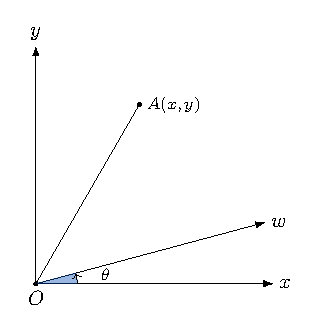
\includegraphics[width=\textwidth]{Chapter2/figure9a.pdf}
		\end{minipage}%
	\hfill
		\begin{minipage}[b]{0.48\textwidth} % Top-right image
		    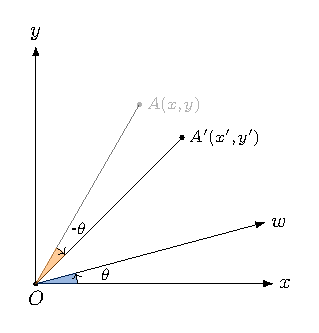
\includegraphics[width=\textwidth]{Chapter2/figure9b.pdf}
		\end{minipage}
	\end{center}
\caption{Παράδειγμα μεταφοράς σχήματος κατά διάνυσμα $v = (t_x, t_y)$}
\end{figure}


\begin{figure}[h!]
	\begin{center}
		\begin{minipage}[b]{0.48\textwidth} % Top-left image
		    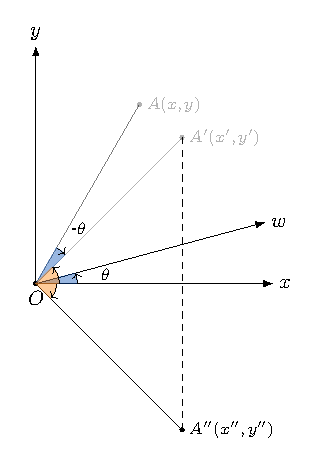
\includegraphics[width=\textwidth]{Chapter2/figure9c.pdf}
		\end{minipage}%
	\hfill
		\begin{minipage}[b]{0.48\textwidth} % Top-right image
		    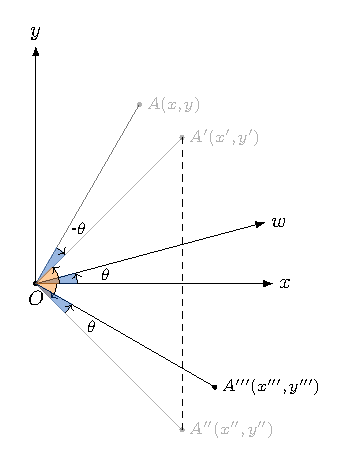
\includegraphics[width=\textwidth]{Chapter2/figure9d.pdf}
		\end{minipage}
	\end{center}
\caption{Παράδειγμα μεταφοράς σχήματος κατά διάνυσμα $v = (t_x, t_y)$}
\end{figure}



Όπως φαίνεται και στο σχήμα \ref{fig:9} ο μετασχηματισμός μπορεί να προκύψει ως εξής:
 
\begin{tabular}{m{0.45\textwidth}m{0.5\textwidth}}
	1. Στροφή της εικόνας κατά γωνία \( -\theta \). & \( (R_{-\theta}) \) \\
	2. Συμμετρία ως προς άξονα $x$.& \( (M_x) \)\\
	3.  Στροφή της εικόνας κατά γωνία \( \theta \).& \( (R_{\theta}) \)
\end{tabular}


\[
\text{Βήμα 1: } 
\begin{bmatrix}
x' \\ y' \\ 1
\end{bmatrix}
=
\begin{bmatrix}
\cos(-\theta) & -\sin(-\theta) & 0 \\
\sin(-\theta) & \cos(-\theta) & 0 \\
0 & 0 & 1
\end{bmatrix}
\cdot
\begin{bmatrix}
x \\ y \\ 1
\end{bmatrix}
= \Pi_1
\begin{bmatrix}
x \\ y \\ 1
\end{bmatrix}
\]

\[
\text{Βήμα 2: } 
\begin{bmatrix}
x'' \\ y'' \\ 1
\end{bmatrix}
=
\begin{bmatrix}
1 & 0 & 0 \\
0 & -1 & 0 \\
0 & 0 & 1
\end{bmatrix}
\cdot
\begin{bmatrix}
x' \\ y' \\ 1
\end{bmatrix}
= \Pi_2
\begin{bmatrix}
x' \\ y' \\ 1
\end{bmatrix}
\]

\[
\text{Βήμα 3: } 
\begin{bmatrix}
x''' \\ y''' \\ 1
\end{bmatrix}
=
\begin{bmatrix}
\cos \theta & -\sin \theta & 0 \\
\sin \theta & \cos \theta & 0 \\
0 & 0 & 1
\end{bmatrix}
\cdot
\begin{bmatrix}
x'' \\ y'' \\ 1
\end{bmatrix}
= \Pi_3
\begin{bmatrix}
x'' \\ y'' \\ 1
\end{bmatrix}
\]

Άρα τελικά:
\[
\begin{bmatrix}
x''' \\ y''' \\ 1
\end{bmatrix}
=
\Pi_3 (\Pi_2 (\Pi_1
\begin{bmatrix}
x \\ y \\ 1
\end{bmatrix}))
\]

Επειδή ο πολλαπλασιασμός πινάκων είναι πράξη προσεταιριστική, θα έχουμε:

\[
\begin{bmatrix}
x''' \\ y''' \\ 1
\end{bmatrix}
=
(\Pi_3 \cdot \Pi_2 \cdot \Pi_1)
\begin{bmatrix}
x \\ y \\ 1
\end{bmatrix}
\]

και επομένως μπορούμε να υπολογίσουμε το γινόμενο $\Pi_3 \Pi_2 \Pi_1$ το οποίο θα αποτελεί και τον ζητούμενο πίνακα $\Pi$.

\[
\Pi =
\begin{bmatrix}
\cos \theta & -\sin \theta & 0 \\
\sin \theta & \cos \theta & 0 \\
0 & 0 & 1
\end{bmatrix}
\cdot
\begin{bmatrix}
1 & 0 & 0 \\
0 & -1 & 0 \\
0 & 0 & 1
\end{bmatrix}
\cdot
\begin{bmatrix}
\cos(-\theta) & -\sin(-\theta) & 0 \\
\sin(-\theta) & \cos(-\theta) & 0 \\
0 & 0 & 1
\end{bmatrix}
\]

\[
=
\begin{bmatrix}
\cos \theta & \sin \theta & 0 \\
-\sin \theta & \cos \theta & 0 \\
0 & 0 & 1
\end{bmatrix}
\cdot
\begin{bmatrix}
\cos \theta & \sin \theta & 0 \\
-\sin \theta & \cos \theta & 0 \\
0 & 0 & 1
\end{bmatrix}
=
\]

\[
\begin{bmatrix}
\cos^2\theta - \sin^2\theta & 2\sin\theta\cos\theta & 0 \\
2\sin\theta\cos\theta & \sin^2\theta - \cos^2\theta & 0 \\
0 & 0 & 1
\end{bmatrix}
\cdot
\begin{bmatrix}
\cos 2\theta & \sin 2\theta & 0 \\
\sin 2\theta & -\cos 2\theta & 0 \\
0 & 0 & 1
\end{bmatrix}
\]

\section{Σύνθεση μετασχηματισμών}

Είναι φανερό ότι κάνοντας χρήση της προσεταιριστικής ιδιότητας του πολλαπλασιασμού πινάκων μπορούμε να παραστήσουμε \textbf{μία ακολουθία μετασχηματισμών} (που εφαρμόζονται πάνω σε μία εικόνα) \textbf{με έναν μόνο πίνακα.}

Έστω γενικά $M_1, M_2, \ldots, M_n$ μετασχηματισμοί που εφαρμόζονται με τη σειρά αυτή πάνω σε μία εικόνα. Οι αντίστοιχοι ομογενείς πίνακες είναι $\Pi_i, i=1(\text{ή } n)$. Ο συνολικός μετασχηματισμός κάθε σημείου της εικόνας μπορεί να υπολογιστεί ως εξής:

\[
\begin{bmatrix}
x' \\ y' \\ 1
\end{bmatrix}
=
\Pi_n (\Pi_{n-1} (\ldots (\Pi_2 (\Pi_1
\begin{bmatrix}
x \\ y \\ 1
\end{bmatrix}))))
=
((\Pi_n \Pi_{n-1}) \Pi_{n-2}) \ldots \Pi_1)
\begin{bmatrix}
x \\ y \\ 1
\end{bmatrix}
\]

ή απλά:

\[
\begin{bmatrix}
x' \\ y' \\ 1
\end{bmatrix}
=
\Pi_n \Pi_{n-1} \Pi_{n-2} \ldots \Pi_1
\begin{bmatrix}
x \\ y \\ 1
\end{bmatrix}
\]

Ο συνολικός μετασχηματισμός λοιπόν παρουσιάζεται με έναν πίνακα ο οποίος υπολογίζεται μία φορά και στη συνέχεια πολλαπλασιάζεται με τα εκάστοτε σημεία της εικόνας.

\section{Παραδείγματα μετασχηματισμών στο επίπεδο}

\begin{example}
Περιγράψτε το μετασχηματισμό που περιστρέφει ένα δοσμένο σημείο $Q(x, y)$ κατά γωνία $\theta$ ως προς ένα δοσμένο κέντρο περιστροφής $P(h, k)$ (σχήμα 3.10). Υπολογίστε το σχετικό πίνακα $R_{\theta, P}$ που θα εκτελεί το συγκεκριμένο μετασχηματισμό.

\begin{figure}[h!]
	\begin{center}
		    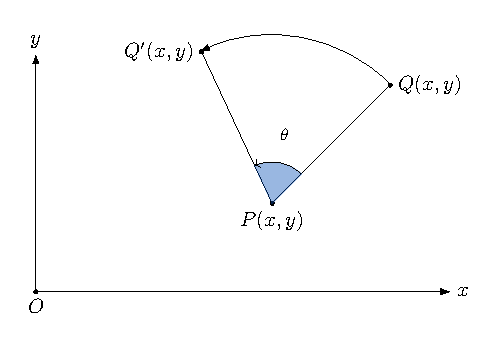
\includegraphics[scale=1]{Chapter2/figure10.pdf}
	\end{center}
	\caption{πίνακας μετασχηματισμού \textcolor{red}{what}}
\end{figure}

\end{example}

\begin{solution}
	


Εφαρμόζουμε γεωμετρικούς μετασχηματισμούς. Θα προσπαθήσουμε να αναγούμε το ζητούμενο μετασχηματισμό σε σύνθεση βασικών μετασχηματισμών. Εκτελούμε τα ακόλουθα βήματα:

Βήμα 1: Μεταφέρουμε το κέντρο περιστροφής $P$ στην αρχή των αξόνων. Η μεταφορά θα γίνει κατά διάνυσμα $V$ όπου $V = -h\hat{i} - k\hat{j}$, όπου $\hat{i}, \hat{j}$ τα μοναδιαία διανύσματα στους άξονες $x$ και $y$ αντίστοιχα (Σχήμα 3.11).

\[
\text{Βασικός πίνακας μετασχηματισμού: } T_v
\]

\begin{figure}[h!]
	\begin{center}
		    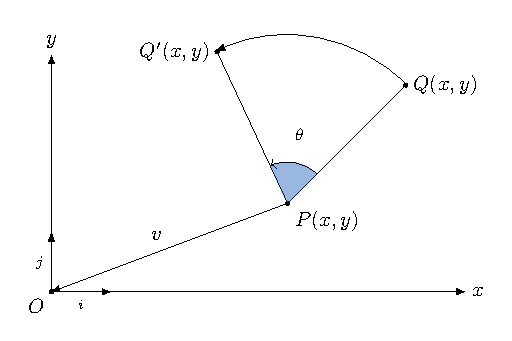
\includegraphics[scale=1]{Chapter2/figure11.pdf}
	\end{center}
	\caption{πίνακας μετασχηματισμού \textcolor{red}{what}}
\end{figure}


Βήμα 2: Εκτελούμε περιστροφή κατά γωνία $\theta$ ως προς την αρχή των αξόνων εφαρμόζοντας το μετασχηματισμό $R_\theta$ (Σχήμα 3.12).

\[
\text{Βασικός πίνακας μετασχηματισμού: } R_\theta
\]

\begin{figure}[h!]
	\begin{center}
		    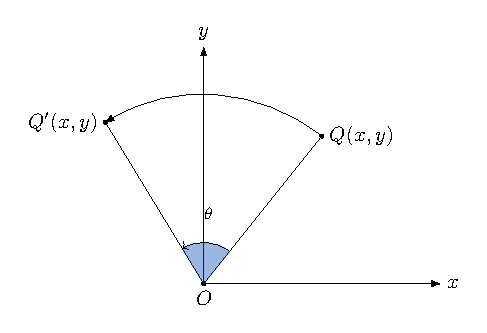
\includegraphics[scale=1]{Chapter2/figure12.pdf}
	\end{center}
	\caption{πίνακας μετασχηματισμού \textcolor{red}{what}}
\end{figure}


Βήμα 3: Μεταφέρουμε το $P$ στην αρχική του θέση. Η μεταφορά θα γίνει κατά διάνυσμα $-V$ (Σχήμα 3.13).

\[
\text{Βασικός πίνακας μετασχηματισμού: } T_{-V}
\]

\begin{figure}[h!]
	\begin{center}
		    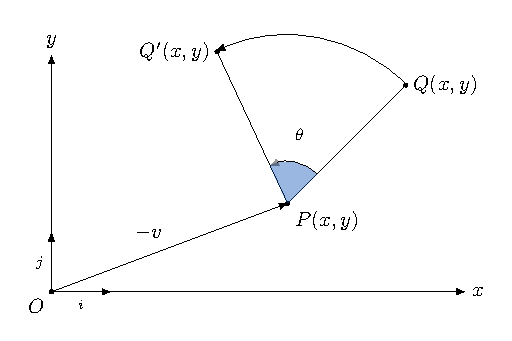
\includegraphics[scale=1]{Chapter2/figure13.pdf}
	\end{center}
	\caption{πίνακας μετασχηματισμού \textcolor{red}{what}}
\end{figure}


Ο ζητούμενος μετασχηματισμός προκύπτει ως σύνθεση των παραπάνω:

\[
R_{\theta,P} = T_{-V} \circ R_\theta \circ T_V
\]

Εφαρμόζοντας τους βασικούς γνωστούς πίνακες προκύπτει ότι:

\[
R_{\theta,P} =
\begin{bmatrix}
1 & 0 & 0 \\
0 & 1 & 0 \\
-h & -k & 1
\end{bmatrix}
\cdot
\begin{bmatrix}
\cos\theta & -\sin\theta & 0 \\
\sin\theta & \cos\theta & 0 \\
0 & 0 & 1
\end{bmatrix}
\cdot
\begin{bmatrix}
1 & 0 & 0 \\
0 & 1 & 0 \\
h & k & 1
\end{bmatrix}
=
\begin{bmatrix}
\cos\theta & -\sin\theta & -h\cos\theta + k\sin\theta + h \\
\sin\theta & \cos\theta & -h\sin\theta - k\cos\theta + k \\
0 & 0 & 1
\end{bmatrix}
\]

Οι συντεταγμένες του καινούργιου σημείου $Q'(x', y')$ προκύπτουν από την επίδραση του $R_{\theta,P}$ πάνω στο αρχικό σημείο $Q(x, y)$:

\[
\text{Τελικά:}
\begin{bmatrix}
x' \\ y' \\ 1
\end{bmatrix}
=
R_{\theta,P}
\begin{bmatrix}
x \\ y \\ 1
\end{bmatrix}
\]
\end{solution}
\begin{example}
Περιγράψτε το μετασχηματισμό $M_L$, που βρίσκεται το συμμετρικό ενός αντικειμένου ως προς μία ευθεία $L$, που τέμνει τον άξονα των $y$ στο $(0,b)$ και σχηματίζει με τον άξονα των $x$ γωνία $\theta$.
\end{example}
\begin{solution}

%\input{figure16}

Εφαρμόζουμε γεωμετρικούς μετασχηματισμούς. Θα προσπαθήσουμε να ανάγουμε το ζητούμενο μετασχηματισμό σε σύνθεση βασικών μετασχηματισμών και ιδιαίτερα της βασικής συμμετρίας ως προς τους άξονες $x$ και $y$. Εκτελούμε τα ακόλουθα βήματα:


Βήμα 1:  Μεταφέρουμε το σημείο $(0, b)$ στην αρχή των αξόνων. Η μεταφορά θα γίνει κατά διάνυσμα $-v$, όπου $v = b\hat{i}$, $\hat{i}$, $\hat{j}$ τα μοναδιαία στους άξονες $x$ και $y$ αντίστοιχα.

\[
\text{Βασικός πίνακας μετασχηματισμού: } T_{-v}
\]

Βήμα 2: Στρέφουμε κατά γωνία $-\theta$ ώστε η ευθεία $L$ να ευθυγραμμιστεί με τον άξονα των $x$.

\[
\text{Βασικός πίνακας μετασχηματισμού: } R_{-\theta}
\]

Βήμα 3: Παίρνουμε το συμμετρικό ως προς τον άξονα των $x$.

\[
\text{Βασικός πίνακας μετασχηματισμού: } M_x
\]

Βήμα 4: Εκτελούμε στροφή κατά γωνία $\theta$.

\[
\text{Βασικός πίνακας μετασχηματισμού: } R_\theta
\]

Βήμα 5: Επαναφέρουμε το σημείο $(O, b)$ στην αρχική του θέση. Η μεταφορά θα γίνει κατά διάνυσμα $v$.


\[
\text{Βασικός πίνακας μετασχηματισμού: } T_v
\]

Ο ζητούμενος μετασχηματισμός θα προκύψει σαν σύνθεση των παραπάνω βασικών μετασχηματισμών.

\[
M_L = T_v \cdot R_{\theta} \cdot M_x \cdot R_{-\theta} \cdot T_{-v} \tag{1}
\]

Εάν τώρα υποθέσουμε ότι η κλίση της ευθείας $L$ είναι $m$, δηλαδή $\tan\theta = m$, και κατά συνέπεια $\sin\theta = \frac{m}{\sqrt{m^2+1}}$, $\cos\theta = \frac{1}{\sqrt{m^2+1}}$, η σχέση (1) γίνεται:

\[
M_L = \begin{bmatrix}
1 & 0 & 0 \\
0 & 1 & b \\
0 & 0 & 1
\end{bmatrix}
\begin{bmatrix}
\cos\theta & -\sin\theta & 0 \\
\sin\theta & \cos\theta & 0 \\
0 & 0 & 1
\end{bmatrix}
\begin{bmatrix}
1 & 0 & 0 \\
0 & -1 & 0 \\
0 & 0 & 1
\end{bmatrix}
\begin{bmatrix}
\cos\theta & \sin\theta & 0 \\
-\sin\theta & \cos\theta & 0 \\
0 & 0 & 1
\end{bmatrix}
\begin{bmatrix}
1 & 0 & 0 \\
0 & 1 & -b \\
0 & 0 & 1
\end{bmatrix}
\]

Με υπολογισμούς προκύπτει:

\[
M_L = \begin{bmatrix}
\frac{1 - m^2}{m^2 + 1} & \frac{2m}{m^2 + 1} & \frac{-2bm}{m^2 + 1} \\
\frac{2m}{m^2 + 1} & \frac{m^2 - 1}{m^2 + 1} & \frac{2b}{m^2 + 1} \\
0 & 0 & 1
\end{bmatrix}
\]
\end{solution}
\begin{example}
Περιγράψτε το μετασχηματισμό που εκτελεί scaling ενός αντικειμένου ως προς ένα δοσμένο σταθερό σημείο $P(h,k)$ (Σχήμα 3.14). Το scaling να γίνει κατά $a$ μονάδες στον άξονα $x$ και κατά $b$ μονάδες στον άξονα $y$. Υπολογίστε το σχετικό πίνακα $S_{a,b,P}$ που θα εκτελεί το συγκεκριμένο μετασχηματισμό.
\end{example}
\begin{solution}

	
\begin{figure}[h!]
	\begin{center}
		\begin{minipage}[b]{0.45\textwidth} % Top-left image
		    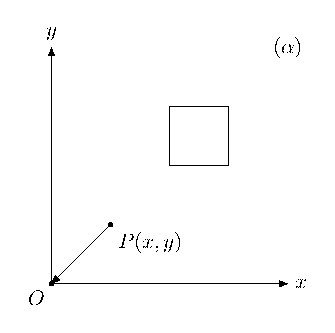
\includegraphics[width=\textwidth]{Chapter2/figure14a.pdf}
		\end{minipage}%
	\hfill
		\begin{minipage}[b]{0.45\textwidth} % Top-right image
		    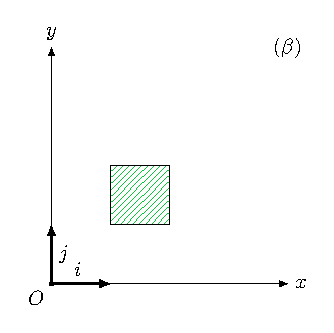
\includegraphics[width=\textwidth]{Chapter2/figure14b.pdf}
		\end{minipage}
	\end{center}
%\caption{Στρέβλωση ενός τετραγώνου για $a=2$ και $b=2$}
\end{figure}

\begin{figure}[h!]
	\begin{center}
		\begin{minipage}[b]{0.45\textwidth} % Top-left image
		    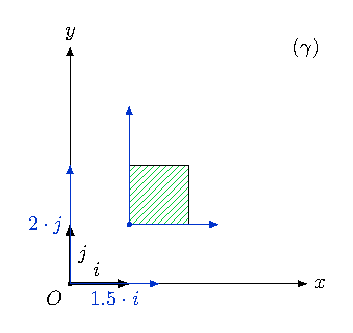
\includegraphics[width=\textwidth]{Chapter2/figure14c.pdf}
		\end{minipage}%
	\hfill
		\begin{minipage}[b]{0.45\textwidth} % Top-right image
		    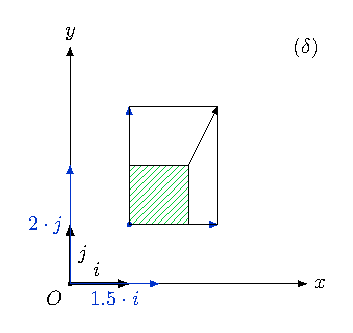
\includegraphics[width=\textwidth]{Chapter2/figure14d.pdf}
		\end{minipage}
	\end{center}
%\caption{Στρέβλωση ενός τετραγώνου για $a=2$ και $b=2$}
\end{figure}

\begin{figure}[h!]
	\begin{center}
		\begin{minipage}[b]{0.45\textwidth} % Top-left image
		    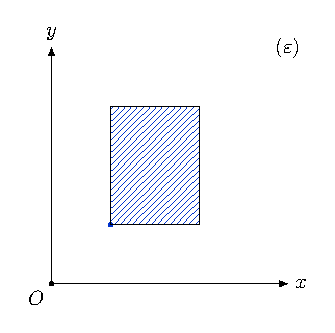
\includegraphics[width=\textwidth]{Chapter2/figure14e.pdf}
		\end{minipage}%
	\hfill
		\begin{minipage}[b]{0.45\textwidth} % Top-right image
		    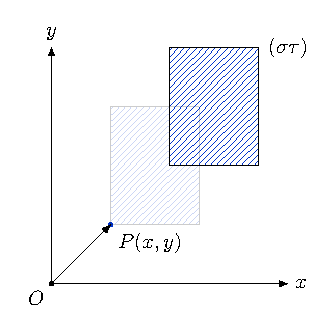
\includegraphics[width=\textwidth]{Chapter2/figure14f.pdf}
		\end{minipage}
	\end{center}
\end{figure}

Εφαρμόζουμε γεωμετρικούς μετασχηματισμούς. Θα προσπαθήσουμε να αναγάγουμε το ζητούμενο μετασχηματισμό σε σύνθεση βασικών μετασχηματισμών και ιδιαίτερα του βασικού scaling ως προς την αρχή των αξόνων. Εκτελούμε τα ακόλουθα βήματα:

Βήμα 1: Μεταφέρουμε το σταθερό σημείο $P$ στην αρχή των αξόνων. Η μεταφορά θα γίνει κατά διάνυσμα $-V$, όπου $V = h\hat{i} + k\hat{j}$, $\hat{i}$ και $\hat{j}$ τα μοναδιαία διανύσματα στους άξονες $x$ και $y$ αντίστοιχα (Σχήμα 3.14(b)).



\[
\text{Βασικός πίνακας μετασχηματισμού:} T_{-V}
\]

Βήμα 2: Εκτελούμε scaling ως προς την αρχή των αξόνων με $s_x = a$ και $s_y = b$ (Σχήμα 3.14(c)).

\[
\text{Βασικός πίνακας μετασχηματισμού: } S_{s_x, s_y}
\]

Βήμα 3: Επαναφέρουμε το σημείο $P$ στην αρχική του θέση. Η μεταφορά θα γίνει τώρα κατά διάνυσμα $V$ (Σχήμα 3.14(d)).

\[
\text{Βασικός πίνακας μετασχηματισμού: } T_V
\]

Ο ζητούμενος μετασχηματισμός θα προκύψει σαν σύνθεση των παραπάνω βασικών μετασχηματισμών:

\[
S_{a,b,P} = T_V \circ S_{s_x, s_y} \circ T_{-V}
\]

Αντικαθιστώντας τους βασικούς πίνακες μετασχηματισμών στην παραπάνω σχέση προκύπτει ότι:

\[
S_{a,b,P} =
\begin{bmatrix}
1 & 0 & h \\
0 & 1 & k \\
0 & 0 & 1
\end{bmatrix}
\cdot
\begin{bmatrix}
a & 0 & 0 \\
0 & b & 0 \\
0 & 0 & 1
\end{bmatrix}
\cdot
\begin{bmatrix}
1 & 0 & -h \\
0 & 1 & -k \\
0 & 0 & 1
\end{bmatrix}
=
\begin{bmatrix}
a & 0 & -ah + h \\
0 & b & -bk + k \\
0 & 0 & 1
\end{bmatrix}
\]

Οι συντεταγμένες των καινούργιων σημείων του αντικειμένου προκύπτουν από την επίδραση του $S_{a,b,P}$ πάνω στο αρχικό αντικείμενο.

Βασική παρατήρηση: Χρησιμοποιώντας το μετασχηματισμό $S_{a,b,P}$ μπορούμε να τροποποιήσουμε τις διαστάσεις ενός αντικειμένου διατηρώντας σταθερό ένα συγκεκριμένο σημείο του $P$.
\end{solution}
\begin{example}
Περιγράψτε το μετασχηματισμό που εκτελεί scaling ενός αντικειμένου ως προς ένα δοσμένο σταθερό σημείο $P(h,k)$ (Σχήμα 3.14). Το scaling να γίνει κατά $a$ μονάδες στον άξονα $x$ και κατά $b$ μονάδες στον άξονα $y$. Υπολογίστε το σχετικό πίνακα $S_{a,b,P}$ που θα εκτελεί το συγκεκριμένο μετασχηματισμό.
\end{example}
\begin{solution}

	
%\input{figure14}

Εφαρμόζουμε γεωμετρικούς μετασχηματισμούς. Θα προσπαθήσουμε να αναγάγουμε το ζητούμενο μετασχηματισμό σε σύνθεση βασικών μετασχηματισμών και ιδιαίτερα του βασικού scaling ως προς την αρχή των αξόνων. Εκτελούμε τα ακόλουθα βήματα:

Βήμα 1: Μεταφέρουμε το σταθερό σημείο $P$ στην αρχή των αξόνων. Η μεταφορά θα γίνει κατά διάνυσμα $-V$, όπου $V = h\hat{i} + k\hat{j}$, $\hat{i}$ και $\hat{j}$ τα μοναδιαία διανύσματα στους άξονες $x$ και $y$ αντίστοιχα (Σχήμα 3.14(b)).



\[
\text{Βασικός πίνακας μετασχηματισμού:} T_{-V}
\]

Βήμα 2: Εκτελούμε scaling ως προς την αρχή των αξόνων με $s_x = a$ και $s_y = b$ (Σχήμα 3.14(c)).

\[
\text{Βασικός πίνακας μετασχηματισμού: } S_{s_x, s_y}
\]

Βήμα 3: Επαναφέρουμε το σημείο $P$ στην αρχική του θέση. Η μεταφορά θα γίνει τώρα κατά διάνυσμα $V$ (Σχήμα 3.14(d)).

\[
\text{Βασικός πίνακας μετασχηματισμού: } T_V
\]

Ο ζητούμενος μετασχηματισμός θα προκύψει σαν σύνθεση των παραπάνω βασικών μετασχηματισμών:

\[
S_{a,b,P} = T_V \circ S_{s_x, s_y} \circ T_{-V}
\]

Αντικαθιστώντας τους βασικούς πίνακες μετασχηματισμών στην παραπάνω σχέση προκύπτει ότι:

\[
S_{a,b,P} =
\begin{bmatrix}
1 & 0 & h \\
0 & 1 & k \\
0 & 0 & 1
\end{bmatrix}
\cdot
\begin{bmatrix}
a & 0 & 0 \\
0 & b & 0 \\
0 & 0 & 1
\end{bmatrix}
\cdot
\begin{bmatrix}
1 & 0 & -h \\
0 & 1 & -k \\
0 & 0 & 1
\end{bmatrix}
=
\begin{bmatrix}
a & 0 & -ah + h \\
0 & b & -bk + k \\
0 & 0 & 1
\end{bmatrix}
\]

Οι συντεταγμένες των καινούργιων σημείων του αντικειμένου προκύπτουν από την επίδραση του $S_{a,b,P}$ πάνω στο αρχικό αντικείμενο.

Βασική παρατήρηση: Χρησιμοποιώντας το μετασχηματισμό $S_{a,b,P}$ μπορούμε να τροποποιήσουμε τις διαστάσεις ενός αντικειμένου διατηρώντας σταθερό ένα συγκεκριμένο σημείο του $P$.
\end{solution}

\begin{example}
Περιγράψτε το μετασχηματισμό $M_L$, που βρίσκει το συμμετρικό ενός αντικειμένου ως προς μία ευθεία $L$, που τέμνει τον άξονα των $y$ στο $(0,b)$ και σχηματίζει με τον άξονα των $x$ γωνία $\theta$.
\end{example}
\begin{solution}



Εφαρμόζουμε γεωμετρικούς μετασχηματισμούς. Θα προσπαθήσουμε να ανάγουμε το ζητούμενο μετασχηματισμό σε σύνθεση βασικών μετασχηματισμών και ιδιαίτερα της βασικής συμμετρίας ως προς τους άξονες $x$ και $y$. Εκτελούμε τα ακόλουθα βήματα:


Βήμα 1:  Μεταφέρουμε το σημείο $(0, b)$ στην αρχή των αξόνων. Η μεταφορά θα γίνει κατά διάνυσμα $-v$, όπου $v = b\hat{i}$, $\hat{i}$, $\hat{j}$ τα μοναδιαία στους άξονες $x$ και $y$ αντίστοιχα.

Βήμα 2: Στρέφουμε κατά γωνία $-\theta$ ώστε η ευθεία $L$ να ευθυγραμμιστεί με τον άξονα των $x$.

\begin{figure}[h!]
	\begin{center}
		\begin{minipage}[b]{0.48\textwidth} % Top-left image
		%    \centering
		    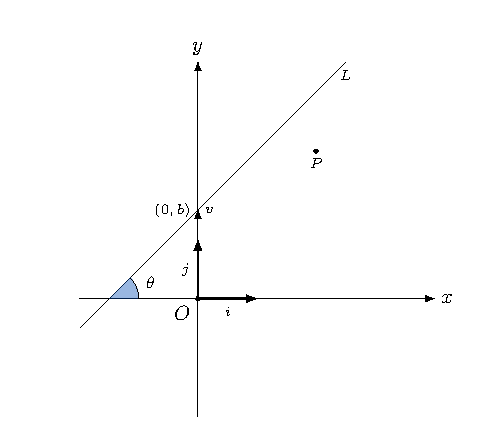
\includegraphics[scale=1]{Chapter2/figure16a.pdf}
		    \captionof{figure}{Βήμα 1: Βασικός μετασχηματισμός $T_{-v}$}
		\end{minipage}%
	\hfill
		\begin{minipage}[b]{0.48\textwidth} % Top-right image
		%    \centering
			    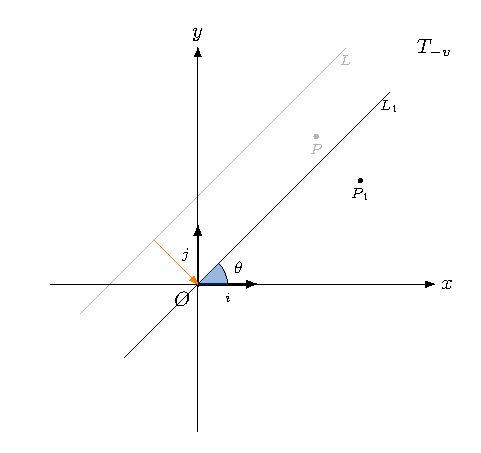
\includegraphics[scale=1]{Chapter2/figure16b.pdf}
		    \captionof{figure}{Βήμα 2: Βασικός μετασχηματισμός $R_{-\theta}$}
		\end{minipage}
	\end{center}
\end{figure}


Βήμα 3: Παίρνουμε το συμμετρικό ως προς τον άξονα των $x$.

Βήμα 4: Εκτελούμε στροφή κατά γωνία $\theta$.


\begin{figure}[h!]
	\begin{center}
		\begin{minipage}[b]{0.48\textwidth} % Top-left image
		%    \centering
		    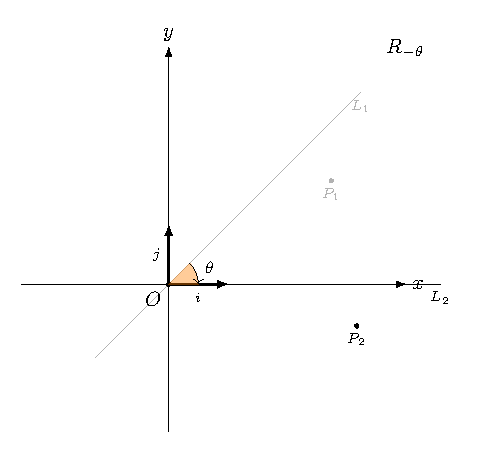
\includegraphics[scale=1]{Chapter2/figure16c.pdf}
		    \captionof{figure}{Βήμα 3: Βασικός μετασχηματισμός $M_x$}
		\end{minipage}%
	\hfill
		\begin{minipage}[b]{0.48\textwidth} % Top-right image
		%    \centering
			    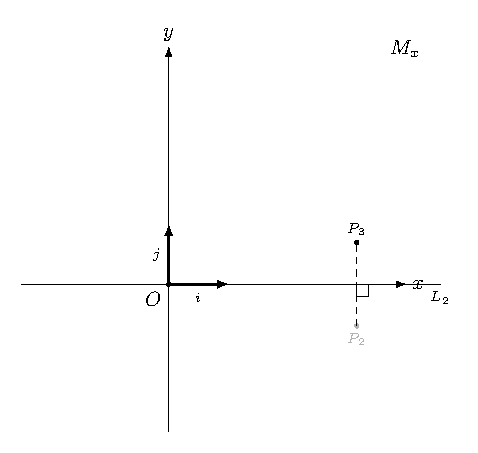
\includegraphics[scale=1]{Chapter2/figure16d.pdf}
		    \captionof{figure}{Βήμα 4: Βασικός μετασχηματισμός $R_{\theta}$}
		\end{minipage}
	\end{center}
\end{figure}


Βήμα 5: \textcolor{red}{Συμμετρικό} ως προς άξονα $x$.






Βήμα 6: Επαναφέρουμε το σημείο $(O, b)$ στην αρχική του θέση. Η μεταφορά θα γίνει κατά διάνυσμα $v$.



\begin{figure}[h!]
	\begin{center}
		\begin{minipage}[b]{0.48\textwidth} % Top-left image
		%    \centering
		    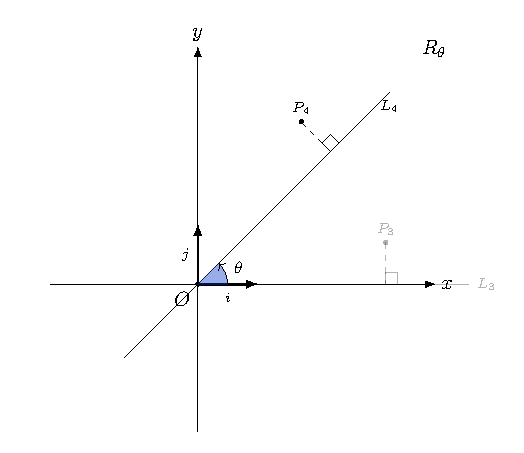
\includegraphics[scale=1]{Chapter2/figure16e.pdf}
		    \captionof{figure}{Βήμα 5: Βασικός μετασχηματισμός $M_x$}
		\end{minipage}%
	\hfill
		\begin{minipage}[b]{0.48\textwidth} % Top-right image
		%    \centering
			    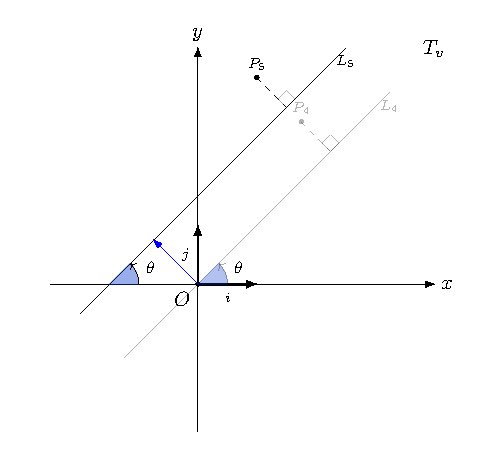
\includegraphics[scale=1]{Chapter2/figure16f.pdf}
		    \captionof{figure}{Βήμα 4: Βασικός μετασχηματισμός $T_v$}
		\end{minipage}
	\end{center}
\end{figure}


Ο ζητούμενος μετασχηματισμός θα προκύψει σαν σύνθεση των παραπάνω βασικών μετασχηματισμών.

\[
M_L = T_v \cdot R_{\theta} \cdot M_x \cdot R_{-\theta} \cdot T_{-v} \tag{1}
\]

Εάν τώρα υποθέσουμε ότι η κλίση της ευθείας $L$ είναι $m$, δηλαδή $\tan\theta = m$, και κατά συνέπεια $\sin\theta = \cfrac{m}{\sqrt{m^2+1}}$, $\cos\theta = \cfrac{1}{\sqrt{m^2+1}}$, η σχέση (1) γίνεται:

\[
M_L = \begin{bmatrix}
1 & 0 & 0 \\
0 & 1 & b \\
0 & 0 & 1
\end{bmatrix}
\begin{bmatrix}
\cos\theta & -\sin\theta & 0 \\
\sin\theta & \cos\theta & 0 \\
0 & 0 & 1
\end{bmatrix}
\begin{bmatrix}
1 & 0 & 0 \\
0 & -1 & 0 \\
0 & 0 & 1
\end{bmatrix}
\begin{bmatrix}
\cos\theta & \sin\theta & 0 \\
-\sin\theta & \cos\theta & 0 \\
0 & 0 & 1
\end{bmatrix}
\begin{bmatrix}
1 & 0 & 0 \\
0 & 1 & -b \\
0 & 0 & 1
\end{bmatrix}
\]

Με υπολογισμούς προκύπτει:

\[
M_L = \begin{bmatrix}
\cfrac{1 - m^2}{m^2 + 1} & \cfrac{2m}{m^2 + 1} & \cfrac{-2bm}{m^2 + 1} \\
\cfrac{2m}{m^2 + 1} & \cfrac{m^2 - 1}{m^2 + 1} & \cfrac{2b}{m^2 + 1} \\
0 & 0 & 1
\end{bmatrix}
\]
\end{solution}
\begin{example}
 Βρείτε το συμμετρικό του πολυγώνου $V$ με κορυφές $A(-1, 0)$, $B(0, -2)$, $C(1, 0)$ και $D(0, 2)$ ως προς:
\begin{enumerate}
    \item[α)] οριζόντια ευθεία $y=2$
    \item[β)] κατακόρυφη ευθεία $x=2$
    \item[γ)] ευθεία $y=x+2$
\end{enumerate}
\end{example}


\begin{solution}
Το πολύγωνο παρουσιάζεται υπό μορφή πίνακα ως εξής:

\[
V = \begin{bmatrix}
-1 & 0 & 1 & 0 \\
0 & -2 & 0 & 2 \\
1 & 1 & 1 & 1
\end{bmatrix}
\]

Θα χρησιμοποιήσουμε τον πίνακα $M_L$ όπως έχει ορισθεί στο Παράδειγμα 5.\\
α) Η ευθεία $y=2$ έχει σημείο τομής με τον άξονα των $y$ το $(0,2)$ και σχηματίζει γωνία $\theta = 0$ με τον $x$. Επομένως $\theta=0$, $m=0$ και $v=2\hat{j}$. Αντικαθιστώντας αυτές τις τιμές στον πίνακα $M_l$ προκύπτει:
    \[
    M_L = \begin{bmatrix}
    1 & 0 & 0 \\
    0 & -1 & 4 \\
    0 & 0 & 1
    \end{bmatrix}
    \]
Αυτός ο πίνακας αναστρέφει το πολύγωνο συμμετρικά ως προς $y=2$.
Οι συντεταγμένες του καινούργιου πολυγώνου προκύπτουν από τη σχέση:

\[
V' = A'B'C'D' = M_L \cdot V = \begin{bmatrix}
1 & 0 & 0 \\
0 & -1 & 4 \\
0 & 0 & 1
\end{bmatrix}
\begin{bmatrix}
-1 & 0 & 1 & 0 \\
0 & -2 & 0 & 2 \\
1 & 1 & 1 & 1
\end{bmatrix}
= \begin{bmatrix}
-1 & 0 & 1 & 0 \\
4 & 6 & 4 & 2 \\
1 & 1 & 1 & 1
\end{bmatrix}
\]

Τελικό $A' = (-1, 4)$, $B' = (0, 6)$, $C' = (1, 4)$ και $D' = (0, 2)$.

β) Η ευθεία $x=2$ (Σχήμα ) είναι παράλληλη με τον άξονα των $y$ άρα δεν έχει σημείο τομής. Επίσης, έχει άπειρη κλίση! Γι' αυτό αν $v = 2\hat{i}$ θα πρέπει να εκτελεστεί ο ακόλουθος μετασχηματισμός:\\
Βήμα 1: Μεταφορά κατά διάνυσμα $-v$, ώστε η ευθεία $x=2$ να πάει πάνω στον άξονα $y$.
\[
\text{Βασικός πίνακας μετασχηματισμού: } T_{-v}
\]
Βήμα 2: Συμμετρία ως προς $y$.
\[
\text{Βασικός πίνακας μετασχηματισμού: } M_y
\]
Βήμα 3: Επαναφορά της ευθείας $x=2$ στην αρχική της θέση, δηλαδή μεταφορά κατά διάνυσμα $v$.
\[
\text{Βασικός πίνακας μετασχηματισμού: } T_v
\]

Ο ζητούμενος μετασχηματισμός $M$ προκύπτει σαν σύνθεση των παραπάνω, δηλαδή:

\[
M = T_v \cdot M_y \cdot T_{-v} = \begin{bmatrix}
1 & 0 & 2 \\
0 & 1 & 0 \\
0 & 0 & 1
\end{bmatrix}
\begin{bmatrix}
1 & 0 & 0 \\
0 & -1 & 0 \\
0 & 0 & 1
\end{bmatrix}
\begin{bmatrix}
1 & 0 & -2 \\
0 & 1 & 0 \\
0 & 0 & 1
\end{bmatrix} = \begin{bmatrix}
1 & 0 & 0 \\
0 & -1 & 0 \\
0 & 0 & 1
\end{bmatrix}
\]

Οι συντεταγμένες του καινούργιου πολυγώνου δίνονται από:
\[
V' = A'B'C'D' = MV = \begin{bmatrix}
1 & 0 & 0 \\
0 & -1 & 0 \\
0 & 0 & 1
\end{bmatrix}
\begin{bmatrix}
-1 & 0 & 1 & 0 \\
0 & 2 & 0 & 2 \\
1 & 1 & 1 & 1
\end{bmatrix} = \begin{bmatrix}
-1 & 0 & 1 & 0 \\
0 & -2 & 0 & -2 \\
1 & 1 & 1 & 1
\end{bmatrix}
\]

Τελικό $A' = (-1, 0)$, $B' = (0, -2)$, $C' = (1, 0)$ και $D' = (0, -2)$.

γ) Η ευθεία $y=x+2$ έχει κλίση $m=1$ και σημείο τομής με τον άξονα των $y$ το $(0,2)$, επομένως $b=2$. Ο πίνακας $M_l$ του παραδείγματος 5 παίρνει την ακόλουθη τιμή:
\[
M_l = \begin{bmatrix}
0 & 1 & -2 \\
1 & 0 & 2 \\
0 & 0 & 1
\end{bmatrix}
\]

Οι συντεταγμένες του καινούργιου πολυγώνου δίνονται από:
\[
V' = A'B'C'D' = M_l V = \begin{bmatrix}
0 & 1 & -2 \\
1 & 0 & 2 \\
0 & 0 & 1
\end{bmatrix}
\begin{bmatrix}
-1 & 0 & 1 & 0 \\
0 & 2 & 0 & 2 \\
1 & 1 & 1 & 1
\end{bmatrix} = \begin{bmatrix}
2 & 2 & 0 & 2 \\
-1 & 0 & -2 & 0 \\
1 & 1 & 1 & 1
\end{bmatrix}
\]

Τελικό $A' = (2, -1)$, $B' = (2, 0)$, $C' = (0, -2)$ και $D' = (2, 0)$.

Μια στρέβλωση (shearing) κατά μήκος του $X$-άξονα, του σημείου $\overline{P}(x, y)$ με παράγοντα στρέβλωσης $a$, φέρνει το σημείο $\overline{P}$ στο $\overline{P'}(x', y')$ και ισχύει:
\[
x' = x + ay, \quad y' = y .
\]

Χρησιμοποιώντας πίνακες γράφουμε:
\[
\begin{bmatrix}
x' \\
y'
\end{bmatrix} = \begin{bmatrix}
1 & a \\
0 & 1
\end{bmatrix}
\begin{bmatrix}
x \\
y
\end{bmatrix}
\]

ή \(\overline{P'} = SH_x \cdot \overline{P}\) με:
\[
SH_x = \begin{bmatrix}
1 & a \\
0 & 1
\end{bmatrix}
\]

Για την περίπτωση της στρέβλωσης κατά μήκος του $Y$-άξονα και με παράγοντα στρέβλωσης $b$ ισχύει:
\[
SH_y = \begin{bmatrix}
1 & 0 \\
b & 1
\end{bmatrix}
\]


Στο σχήμα  δείχνεται η στρέβλωση ενός τετραγώνου για τις δύο περιπτώσεις $a=2$ και $b=2$.

\begin{figure}[h!]
	\begin{center}
		\begin{minipage}[b]{0.19\textwidth} % Top-left image
		    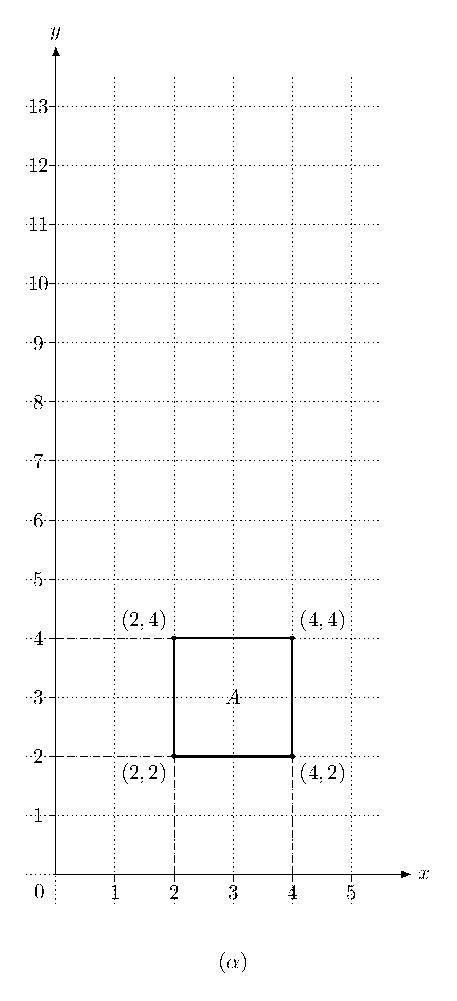
\includegraphics[width=\textwidth]{Chapter2/figure17a.pdf}
		\end{minipage}%
	\hfill
		\begin{minipage}[b]{0.4\textwidth} % Top-right image
		    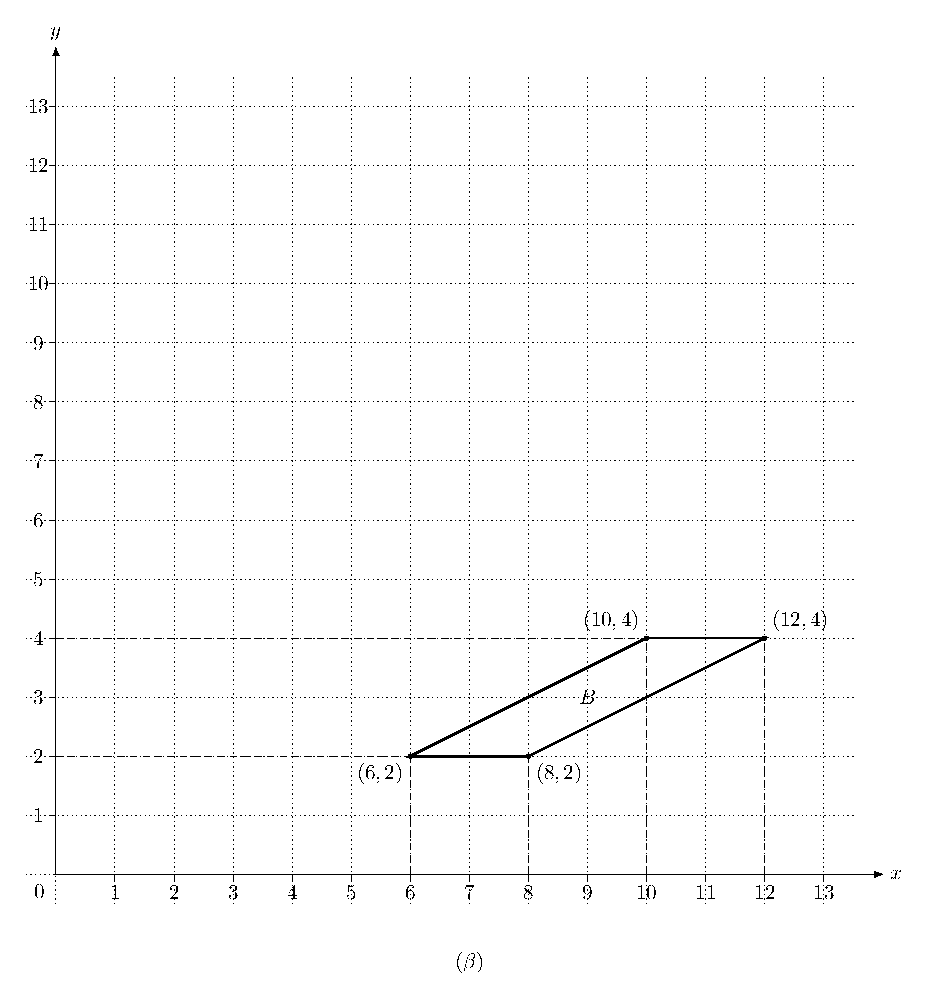
\includegraphics[width=\textwidth]{Chapter2/figure17b.pdf}
		\end{minipage}
	\hfill
		\begin{minipage}[b]{0.4\textwidth} % Top-right image
		    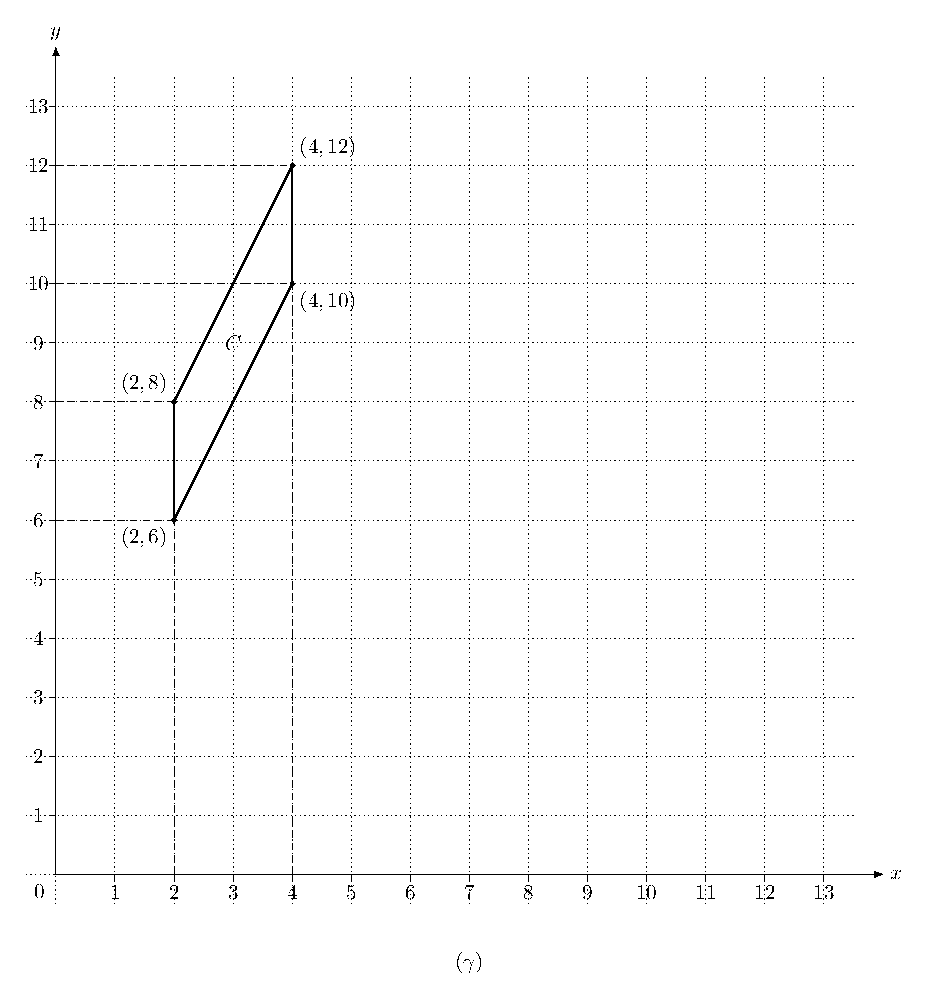
\includegraphics[width=\textwidth]{Chapter2/figure17c.pdf}
		\end{minipage}
	\end{center}
\caption{Στρέβλωση ενός τετραγώνου για $a=2$ και $b=2$}
\end{figure}

\end{solution}





\section*{Ασκήσεις 1ου Κεφαλαίου}

\begin{exercise}
Δίνονται οι εικόνες (α) και (β). Με ποια σύνθεση μετασχηματισμών μπορεί να φέρουμε την εικόνα (α), (β) στη θέση (γ).

%\input{figure18}

\end{exercise}

\begin{solution}
Πρώτα στην εικόνα (α) μπορούμε να δράσουμε ως εξής:
\begin{enumerate}
    \item Σύμπτυξη στις $x$-συντεταγμένες με: \(s_x = \frac{1}{2}\), \(s_y = 1\) (ως προς την αρχή των αξόνων).
    \item Μεταφορά κατά \(\vec{v} = (\frac{3}{2},1) \).
\end{enumerate}

Έτσι, παίρνουμε τον πίνακα μετασχηματισμού:
\[
M_{(a)} = T_v \cdot S_{\frac{1}{2},1} = \begin{bmatrix}
1 & 0 & \frac{3}{2} \\
0 & 1 & 1 \\
0 & 0 & 1
\end{bmatrix}
\begin{bmatrix}
\frac{1}{2} & 0 & 0 \\
0 & 1 & 0 \\
0 & 0 & 1
\end{bmatrix} = \begin{bmatrix}
\frac{1}{2} & 0 & \frac{3}{2} \\
0 & 1 & 1 \\
0 & 0 & 1
\end{bmatrix}
\]

Πράξεις:
\[
\begin{bmatrix}
\frac{1}{2} & 0 & \frac{3}{2} \\
0 & 1 & 1 \\
0 & 0 & 1
\end{bmatrix}
\begin{bmatrix}
-1 & 1 & 0 \\
0 & 0 & 1 \\
1 & 1 & 1
\end{bmatrix} = \begin{bmatrix}
1 & 2 & \frac{3}{2} \\
1 & 1 & 2 \\
1 & 1 & 1
\end{bmatrix}
\]


Αν στην εικόνα (β) μεταφερθεί κατά \(\vec{v} = (1,1)\), θα πάρουμε το τετράγωνο της εικόνας (γ):
\[
\begin{bmatrix}
1 & 0 & 1 \\
0 & 1 & 1 \\
0 & 0 & 1
\end{bmatrix}
\begin{bmatrix}
0 & 1 & 1 & 0 \\
1 & 0 & 1 & 1 \\
1 & 1 & 1 & 1
\end{bmatrix} = \begin{bmatrix}
1 & 2 & 2 & 1 \\
2 & 1 & 2 & 2 \\
1 & 1 & 1 & 1
\end{bmatrix}
\]

\end{solution}

\begin{exercise}
	Ο πίνακας ορίζει ένα μετασχηματισμό που ονομάζεται Shearing. Για $b = 0$, έχουμε shearing στην κατεύθυνση $x$ ενώ για $a=0$ έχουμε shearing στην κατεύθυνση $y$. Με τη βοήθεια αυτού, να βρεθεί ο μετασχηματισμός $M$ που μετατρέπει τον ρόμβο με κορυφές $A (0, \sqrt{2}), B(\sqrt{2},0), \Gamma (0, -\sqrt{2}, \Delta(-\sqrt{2},0)$ στο παραλληλόγραμμο με κορυφές $A^{'} (0,1), B^{'} (1,1), \Gamma^{'}(0,-1), \Delta^{'}$ όπως φαίνεται παρακάτω.

\begin{figure}[h!]
	\begin{center}
		\begin{minipage}[b]{0.4\textwidth} % Top-left image
		    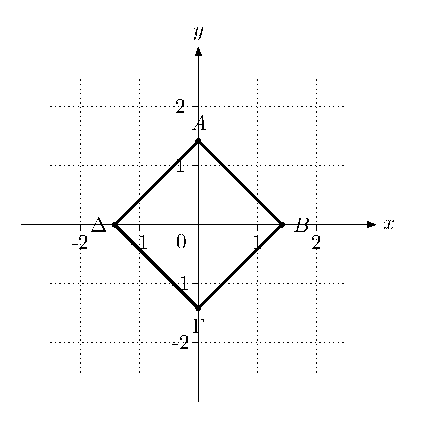
\includegraphics[width=\textwidth]{Chapter2/Exercises/ex2-graph1.pdf}
		\end{minipage}%
	\hfill
		\begin{minipage}[b]{0.4\textwidth} % Top-right image
		    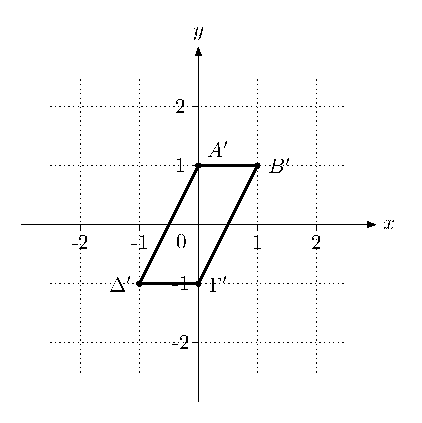
\includegraphics[width=\textwidth]{Chapter2/Exercises/ex2-graph2.pdf}
		\end{minipage}
	\end{center}
%\caption{.}
\end{figure}	
	
\end{exercise}


\begin{solution}

\textbf{\underline{1ος τρόπος}}: 

\begin{enumerate}
	  \item Scaling κατά $S_x = S_y = \cfrac{1}{\sqrt{2}}$ (Πολλαπλασιασμός με πίνακα $S_{S_x, S_y}$)
	  \item Shearing στο $y$ με $b=1$ (Πολλαπλασιασμός με πίνακα $Sh_y$)
\end{enumerate}

\[
	M = 
		\begin{bmatrix}
			1 & 0 \\
			1 & 1
		\end{bmatrix}
	\cdot
		\begin{bmatrix}
			\cfrac{1}{\sqrt{2}} & 0 \\
			0 & \cfrac{1}{\sqrt{2}}
		\end{bmatrix}
	=	
		\begin{bmatrix}
			\cfrac{1}{\sqrt{2}} & 0 \\
			 \cfrac{1}{\sqrt{2}} & \cfrac{1}{\sqrt{2}}
		\end{bmatrix}
	=
	\begin{bmatrix}
			\cfrac{\sqrt{2}}{2} & 0 \\
			 \cfrac{\sqrt{2}}{2} & \cfrac{\sqrt{2}}{2}
		\end{bmatrix}	
\]

Για να υπολογίσουμε πώς ο παραπάνω μετασχηματισμός επιδράσει στο σχήμα $A (0, \sqrt{2}), B(\sqrt{2},0), \Gamma (0, -\sqrt{2}, \Delta(-\sqrt{2},0)$, θα πολλαπλασιάσουμε τον πίνακα τον συντεταγμένων του σχήματος με τον πίνακα του μετασχηματισμού

\[
M \cdot V = 
	\begin{bmatrix}
		\frac{1}{\sqrt{2}} & 0 \\
		\frac{1}{\sqrt{2}} & \frac{1}{\sqrt{2}} 
	\end{bmatrix}
\cdot 
	\begin{bmatrix}
		0 & \sqrt{2} & 0 & -\sqrt{2} \\
		\sqrt{2} & 0 & -\sqrt{2} & 0 
	\end{bmatrix}
	=
	\begin{bmatrix}
		0 & 1 & 0 & -1 \\
		1 & 1 & -1 & -1
	\end{bmatrix}	
\]


\textbf{\underline{2ος τρόπος}}: 

\begin{enumerate}
	  \item Στροφή κατά γωνία $45^\circ$ (Πολλαπλασιασμός με πίνακα $R_{45^\circ}$)
	  \item Scaling $S_x = \cfrac{1}{2}, S_y  = 1$ (Πολλαπλασιασμός με πίνακα $S_{S_x, S_y}$)
	  \item Shearing $S_{h_x}, a = \cfrac{1}{2}, b=0$ (Πολλαπλασιασμός με πίνακα $S_{h_x}$) 
\end{enumerate}

Για να υπολογίσουμε πώς ο παραπάνω μετασχηματισμός επιδράσει στο σχήμα $A (0, \sqrt{2}), B(\sqrt{2},0), \Gamma (0, -\sqrt{2}, \Delta(-\sqrt{2},0)$, θα πολλαπλασιάσουμε τον πίνακα τον συντεταγμένων του σχήματος με τον πίνακα του μετασχηματισμού, δηλαδή με τον πίνακα:

\[
	M = S_{h_x} \cdot S_{S_x, S_y} \cdot R_{\theta}  = 
	\begin{bmatrix}
		1 & \frac{1}{\sqrt{2}} \\
		0 & 1 
	\end{bmatrix}
\cdot 
	\begin{bmatrix}
		\frac{1}{\sqrt{2}} & 0 \\
		0 & 1
	\end{bmatrix}
\cdot
	\begin{bmatrix}
		\cfrac{\sqrt{2}}{2} & -\cfrac{\sqrt{2}}{2} \\
			 \cfrac{\sqrt{2}}{2} & \cfrac{\sqrt{2}}{2}
	\end{bmatrix}	
	=
	\begin{bmatrix}
		\cfrac{\sqrt{2}}{2} & 0 \\
			 \cfrac{\sqrt{2}}{2} & \cfrac{\sqrt{2}}{2}
	\end{bmatrix}
\] 

\end{solution}
\begin{exercise}

Να προσδιοριστούν οι πίνακες στροφής στο χώρο ενός αντικειμένου κατά γωνία $\theta$, ως προς τους άξονες $y'y$, $x'x$, $R_{\theta,y}$ και $R_{\theta,x}$ αντίστοιχα.	
\end{exercise}
\begin{solution}
	



\begin{itemize}
  \item  Για τη στροφή ως προς τον άξονα $y'y$ ισχύουν οι εξής μετασχηματισμοί:
\[
\begin{aligned}
    x' &= x\cos\theta + z\sin\theta, \\
    y' &= y, \\
    z' &= -x\sin\theta + z\cos\theta.
\end{aligned}
\]
Ο αντίστοιχος πίνακας είναι:
\[
R_{\theta,y} = \begin{bmatrix}
\cos\theta & 0 & \sin\theta & 0\\
0 & 1 & 0  & 0\\
-\sin\theta & 0 & \cos\theta & 0\\
0 & 0 & 0 & 1
\end{bmatrix}.
\]

\item Για τη στροφή ως προς τον άξονα $x'x$ ισχύουν οι εξής μετασχηματισμοί:

\[
\begin{aligned}
    x' &= x, \\
    y' &= y\cos\theta - z\sin\theta, \\
    z' &= y\sin\theta + z\cos\theta.
\end{aligned}
\]

Ο αντίστοιχος πίνακας είναι:
\[
R_{\theta,x} = \begin{bmatrix}
1 & 0 & 0 & 0\\
0 & \cos\theta & -\sin\theta & 0\\
0 & \sin\theta & \cos\theta & 0\\
0 & 0 & 0 & 1
\end{bmatrix}.
\]

\end{itemize}
\end{solution}
\begin{exercise}
	Δείξτε ότι ισχύει η αντιμεταθετική ιδιότητα για τα ακόλουθα ζευγάρια μετασχηματισμών.
	\begin{enumerate}
		\item Αν στο χώρο εφαρμόσουμε συμμετρία ως προς το επίπεδο $xy$ και συμμετρία ως προς το επίπεδο $yz$.
		\item Αν στο επίπεδο εφαρμόσουμε μεταφορά κατά διάνυσμα $\vec{v}$ και συμετρία ως προς τον άξονα $y$.
	\end{enumerate}
	
\end{exercise}


%\begin{solution}
%
%\end{solution}
\begin{exercise}
Υπολογίστε στο επίπεδο τον μετασχηματισμό στροφής γωνία $\theta = \cfrac{\pi}{3}$ γύρω από το σημείο $P = (4,1)$

Στην συνέχεια, γράψτε ένα script σε \texttt{Julia} όπου θα υπολογίζει τον παραπάνω πίνακα μετασχηματισμού μέσω πολλαπλασιασμών των βασικών μετασχηματισμών και εφαρμόστε τον, στο παρακάτω σχήμα  σχεδιάζοντας στο ίδιο γράφημα και το αρχικό και το μετασχηματισμένο.

\begin{figure}[hbt]
  \begin{center}
	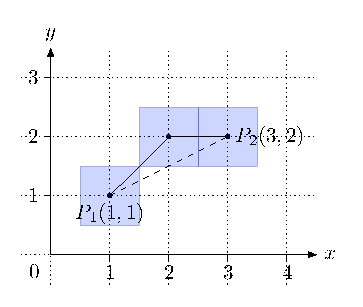
\includegraphics[scale=1]{Chapter1/Exercises/ex17/graph1.pdf}
  \end{center}
%  \caption{Παράσταση ζητούμενων ευθυγ\textcolor{red}{what}ράμμων τμημάτων}
\end{figure}

\end{exercise}
\begin{exercise}

	
\end{exercise}


\begin{solution}

\end{solution}
\begin{exercise}

	
\end{exercise}


\begin{solution}

\end{solution}
\begin{exercise}

	
\end{exercise}


\begin{solution}

\end{solution}
\begin{exercise}

	
\end{exercise}


\begin{solution}

\end{solution}
\begin{exercise}

	
\end{exercise}


\begin{solution}

\end{solution}
\begin{exercise}

	
\end{exercise}


\begin{solution}

\end{solution}
\begin{exercise}

	
\end{exercise}


\begin{solution}

\end{solution}
\begin{exercise}

		
\end{exercise}

\begin{solution}
	
\end{solution}
\begin{exercise}

	
\end{exercise}


\begin{solution}

\end{solution}
